\documentclass{article}
\usepackage[utf8]{inputenc}
\usepackage{romannum}
\usepackage{amsfonts}
\usepackage{amssymb}
\usepackage{fancyhdr}
\usepackage{graphicx}
\usepackage{t1enc}
\usepackage{pdfpages}
\usepackage[magyar]{babel}
\usepackage[utf8]{inputenc}
\usepackage{amsmath}
\usepackage{mathtools}
\usepackage{pdfpages}
\usepackage{ marvosym } 
\usepackage{wrapfig}
\usepackage{hyperref}
\usepackage{pgfplots}

\pgfplotsset{width=\textwidth,compat=newest}
\hypersetup{
    colorlinks,
    citecolor=black,
    filecolor=black,
    linkcolor=black,
    urlcolor=black
}
\usepackage{romannum}
\usepackage{amsfonts}
\usepackage{amssymb}
\usepackage{fancyhdr}
\usepackage{graphicx}
\usepackage{t1enc}
\usepackage{svg}
\usepackage[magyar]{babel}
\usepackage[left=2cm,right=2cm,top=2cm,bottom=2cm]{geometry}

\title{K+F Projekt dokumentáció}
\author{}
\date{2}
\pagestyle{fancy}
\lhead{K+F Projekt dokumentáció}
\rhead{ACSG Kft.}
\cfoot{\thepage. oldal}

\begin{document}
\pagenumbering{arabic}

\begin{center}
    \hrule
    \vspace{0.5cm}
    \begin{Huge}
    K+F projekt dokumentáció\\
    ACSG Kft.\\
    \end{Huge}
    \vspace{0.5cm}
    \begin{huge}
    Időszak:\\
    \end{huge}
    \begin{Large}
    2022.11.01. - 2022.12.31.\\
    \end{Large} \vspace{10pt}
    \begin{large}
    Készítette: Wenesz Dominik\\
    \end{large}\vspace{0.5cm}
    \hrule
    
  \end{center}
  \begin{figure}[b]
    \centering
    
\includegraphics[]{acsg.png}
\end{figure}

  


\thispagestyle{empty}
\setcounter{page}{0}




\newpage
\tableofcontents
\newpage

\section{Összefoglaló}
A dokumentum által specifikált időintervallumban a detektáló rendszerben történtek
főbb előrelépések. Először is a későbbi skálázhatóságra való tekintettel hardveres
területen változtattunk a feldolgozó egységet és kamerarendszert illetőleg. 
Ezenfelül a hagyományos képfeldolgozási módszerek után a mélytanuláson alapuló
módszerek applikálhatóságát vizsgáltuk.\\
A másik terület, melyben munkálatok folytak, az a manipulátor megfogójának
milyenségének kiválasztása, többféle csatlakozóházon való tesztelése. Ez explicit
nem a robotkar pontosságának mérését jelenti, hanem a kereskedelemben fellelhető
végberendezések egymással való összehasonlítását (pl.: strapabíróság, felvehető objektum paraméterei, felvehető objektumok számossága, objektumdetektáló rendszerre 
való illeszthetősége, stb.). A robot pontosságának vizsgálata a következő két hónapos
indőintervallumra esedékes.

\section{Objektum detektáló alrendszer}
\subsection{Hardver változtatások}
Az objektum detektálás szempontjából a Jetson Nano és a RaspberryPi V2.1-es kamera
elegendőnek tekinthető, azonban azon megfontolásból, hogy a későbbiekben 
a rendszer bővíthető legyen, esetlegesen párhuzamosan több feladatot is el
tudjon látni, például egyszerre több különálló kamerakép alapján több 
egymástól független párhuzamos program/algoritmus futhasson párhuzamosan valós
időben, vagy egy komplex, egész gyártócellára kiterjedő optimalizációs rendszer
is futtaható legyen, arra a konklúzióra jutottunk, hogy egy nagyobb erőforrásokkal
rendelkező feldolgozó egységet használunk. Így esett a választás a Jetson Xavier NX-re,
melynek adatlapja megtalálható mellékelve a dokumentációs mappában.\\[5pt]
\begin{figure}[h]
    \centering
    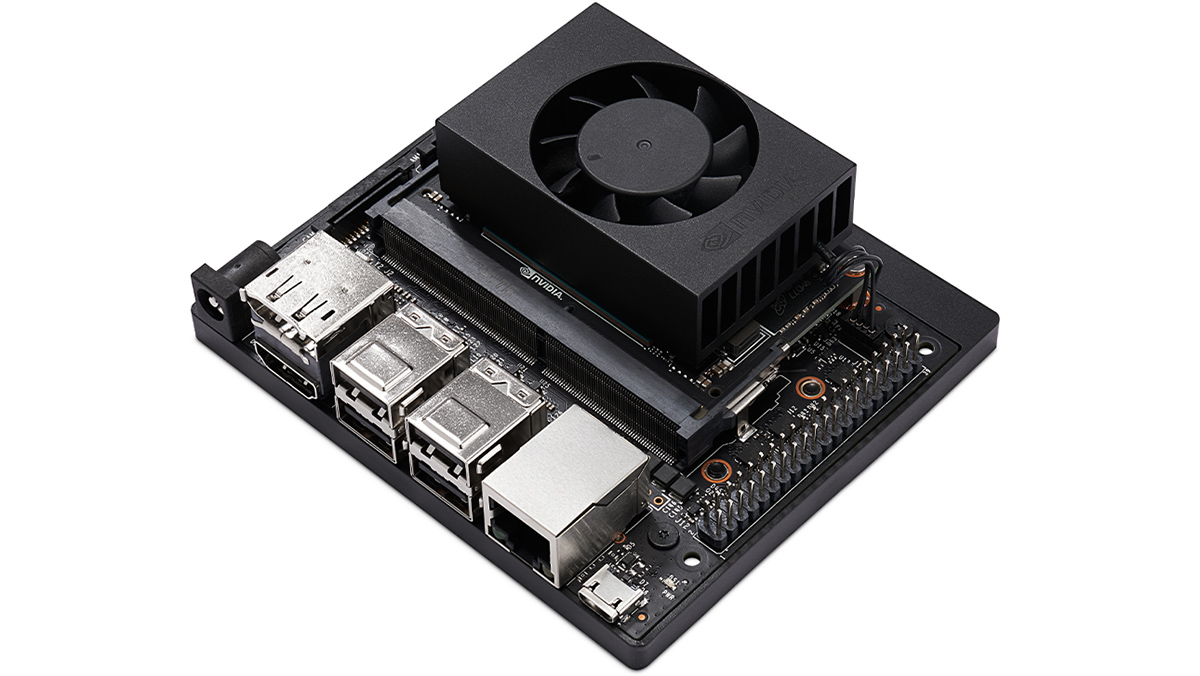
\includegraphics[scale=0.3]{xavier.jpg}
    \caption[]{Jeston Xavier NX Edge System}
\end{figure}\\
Ezen modul előnye, hogy több memóriát, nagyobb számítókapacitású CPU-t és 
nagyobb teljesítményű GPU-t tartalmaz, melyek amint azt későbbiekben láthatjuk 
a mélytanulásos objektumdetektáló módszerekhez elengedhetetlenek.\\[15pt]
A kamera modul választásában szintén változtattunk, mivel a RPi V2.1 képminősége
a kisebb objektumoknál már nem bizonyult megfelelőnek, illetve nem bővíthető
gyárilag lencserendszerrel, így precíz hangolása nehézkes. Ezen indokoknál
fogva választottuk a RaspBerryPi HQ detektort a hozzá tartozó lencserendszerrel 
(optikával) együtt, melyet könnyedén tudunk precízen hangolni. A szenzor és az 
optika adatlapja szintén megtalálható a dokumentáció megfelelő almappájában.\\[5pt]
\begin{figure}[h]
    \centering
    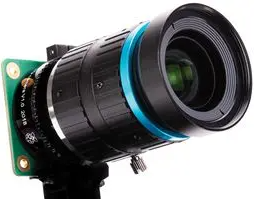
\includegraphics[scale=1]{optika.png}
    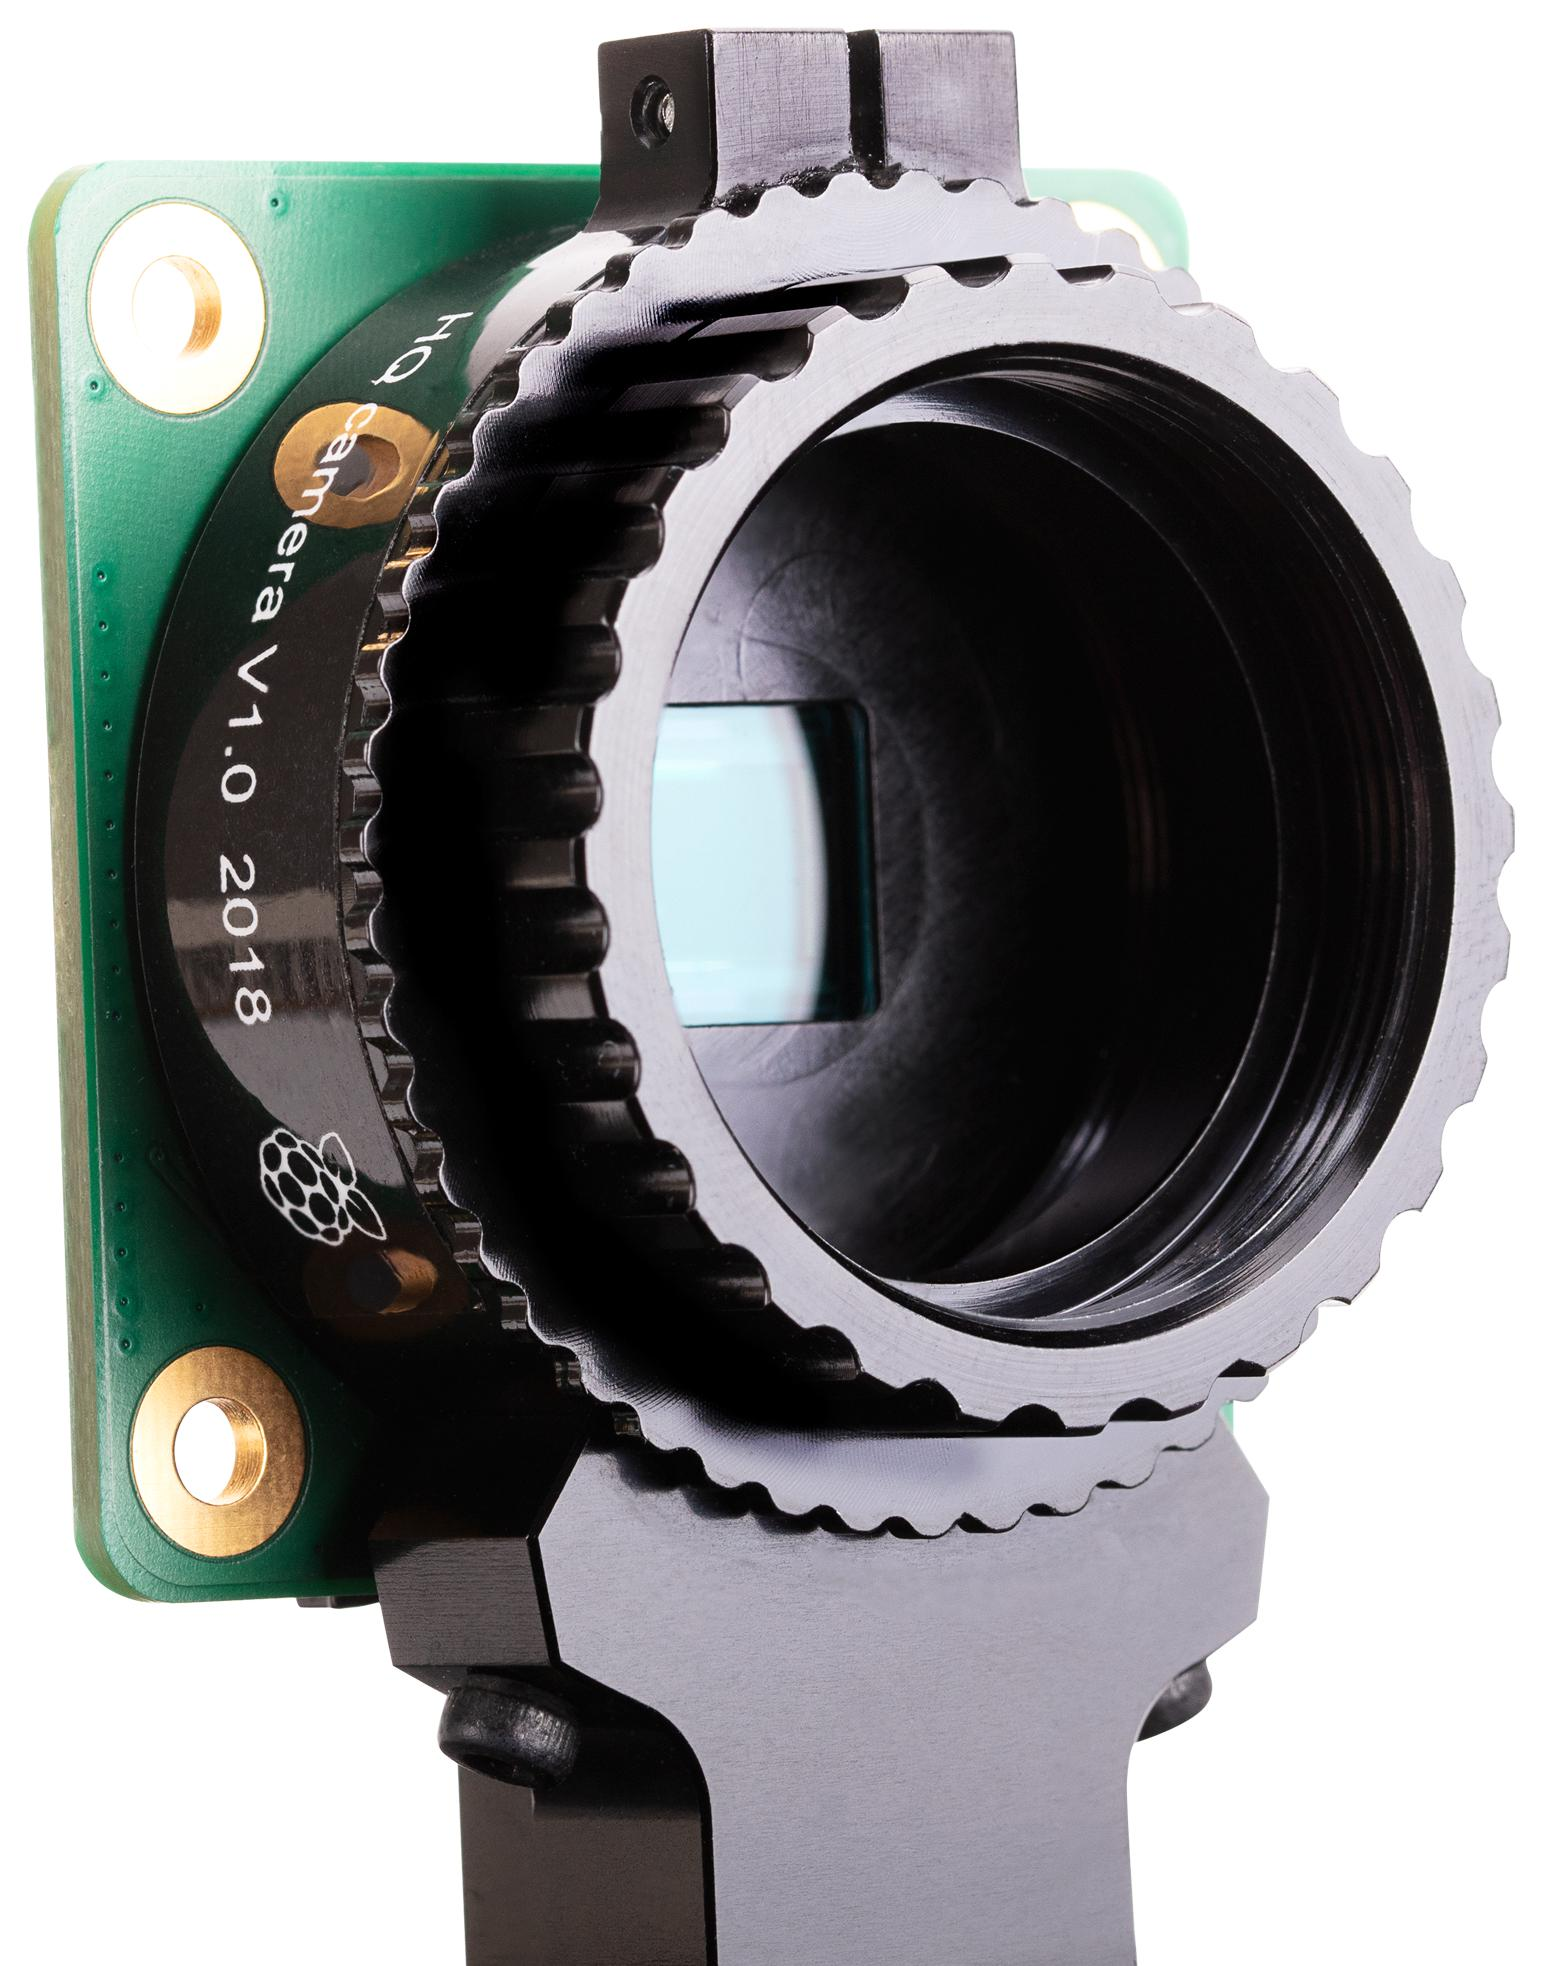
\includegraphics[scale=0.1]{szenzor.jpg}
    \caption{Optikával és optika nélkül felszerelt RPi HQ kamera}
\end{figure}\\

\subsection{Deep Learning}
(leírás +kép)
\subsection{Objektum detektálás mélytanulás alapon}
(leírás + kép)
\subsubsection{Bounding box}
(leírás +kép)
\subsubsection{Semantic segmentation}
(leírás +kép)
\subsubsection{Instance segmentation}
(leírás +kép)
\subsubsection{Keypoint detection}
(leírás +kép)

\subsection{Projekt során nem vizsgálandó hálóarchitektúrák}

\subsection{Vizsgált hálóarchitektúrák}
\subsubsection{Egyszerű konvolúciós háló - U-net}

\subsubsection{SSD}

\subsubsection{YOLO}

\subsection{Konklúzió}

\section{Robot manipulátor}

\subsection{Végberendezés kiválasztása}
(...)

\subsection{Modellezés}
A dokumentum által tárgyalt időszakon belül a használt SCARA robot gépészeti modellezése, jellemző adatainak, melyek
a későbbiekben a szimulációknál, digitális ikernél releváns adatként szolgálhatnak, adatlapból és mérésekből történő 
meghatározása, CAD modell elkészítése, illetőleg a gyártócella hasonló megfontolások alapján történő modellezése 
is megtörtént.\\
(képek...)
\begin{figure}[h]
    \centering
    % na ide jönne mindenféle kép de .stepben egyik alkatrészt sem nyitja meg...
    %\includegraphics[scale = 0.5]{robot.png}
    \caption{CAD modellek}
\end{figure}


\section{Irodalomjegyzék}







\end{document}